% Author: Varsha Ramakrishnan
% Email:vio@berkeley.edu

\qns{Capacitive Touchscreen}

\sol{Prereq: Ability to solve capacitor equivalences.}



Consider the following capacitive touchscreen configuration. (This is a review from lecture.)

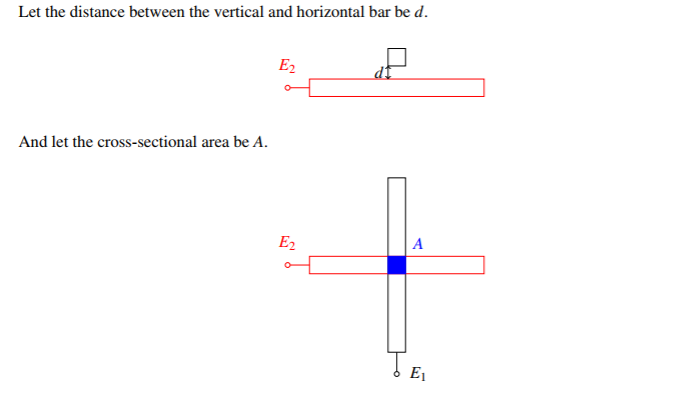
\includegraphics{questions/capacitors.png}

\begin{enumerate}
\qitem{
Draw a diagram representing the capacitance between $E_1$ and $E_2$ when there is no touch on the screen.
}

\ans{

\begin{center}
\begin{circuitikz}
\draw(0,0) 
    to[short, -o, l=$E_1$] ++(0, 0);
\draw(0,0)
	to[C=$C_1$] ++(0,2)
	to[short, -o, l=$E_2$] ++(0,0);

\end{circuitikz}
\end{center}
}

\qitem {
Calculate the value of the capacitance between the two bars when the screen is not being touched.
}
\ans{
$$C_1 = \epsilon A/d$$
}

\qitem{
	Now consider what happens when we touch the screen. Let the blue line represent our finger, and assume there is a capacitance between your finger and each of the bars. The diagram looks like this:
	
	\begin{center}
	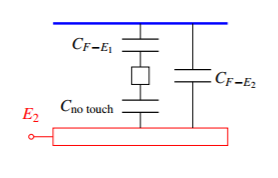
\includegraphics{questions/capacitors_touch.png}
    \end{center}
    Redraw the circuit diagram representing the capacitive touchscreen after being touched, so that the nodes representing $E_1$ and $E_2$ are on opposite ends of the diagram.
    
\begin{center}
\begin{circuitikz}

	
\draw(0,0)
    to[short, -o, l=$E_2$] ++(0, -1);

\draw(0,4)
    to[short, -o, l=$E_1$] ++(0, 1);

\end{circuitikz}
\end{center}
    
}

\ans{
\begin{center}
\begin{circuitikz}
\draw(0,0) 
	to[short] ++(3,0)
	to[C=$C_{F-E_2}$] ++(0,2)
	to node[right] {$\gets$ Finger} ++(0,0)
	to[C=$C_{F-E_1}$] ++(0,2)
	to[short] ++(-3,0)
	to[C=$C_{no\ touch}$] ++(0,-4);
	
\draw(0,0)
    to[short, -o, l=$E_2$] ++(0, -1);

\draw(0,4)
    to[short, -o, l=$E_1$] ++(0, 1);

\end{circuitikz}
\end{center}
}

\qitem{Calculate the new capacitance between $E_1$ and $E_2$. Has it changed from when there was no touch?}

\ans{
Begin by writing the equation that relates all the capacitors using parallel and series symbols, then expand:
\begin{align*}
C_{E_1-E_2}  &= C_{no\ touch} + C_{F-E_1} || C_{F-E_2} \\
&= C_{no\ touch} + \frac{C_{F-E_1}C_{F-E_2}}{C_{F-E_1} + C_{F-E_2}}
\end{align*}
The new capacitance (after touch) is larger than the previous capacitance (before touch). Since the capacitance value has changed by a measurable amount, we can work backwards and find the distance at which the screen was touched.
}


\end{enumerate}